\documentclass[a4paper, 10pt, twocolumn, twoside]{article}

\usepackage{ISARC}

\usepackage{lscape}
\usepackage{hologo}
\usepackage{multirow}

\begin{document}

 % Do not change the following line
\linespread{0.5}

\title{BIM-FM interoperability: integrating existing FM platform with visualization of IFC models}

\author{Andressa Oliveira$^{1}$, José Granja$^1$, Pedro Machado$^2$, Ali Motamedi$^3$, and Miguel Azenha$^1$}

\affiliation{
$^1$University of Minho, ISISE, ARISE, Department of Civil Engineering, Portugal\\
$^2$Matosinhos City Council, Portugal\\
$^2$Université du Québec à Montreal, École de Technologie Supérieure, Canada
}

\email{
\href{mailto:soliveira.andressa@gmail.com}{Email Andressa Oliveira}, 
\href{mailto:granja@civil.uminho.pt}{Email José Granja},
\href{mailto:pedro.machado@cm-matosinhos.pt}{Email Pedro Machado},
\href{mailto:ali.motamedi@etsmtl.ca}{Email Ali Motamedi},
\href{mailto:miguel.azenha@gmail.com}{Email Miguel Azenha}
}


% Do not change the following three lines
\maketitle 
\thispagestyle{fancy} 
\pagestyle{fancy}

\begin{abstract}
The adoption of Building Information Modelling (BIM) in building operations is limited, mostly due to insufficient BIM capabilities in Facility Management (FM) platforms. This article documents the developments from a collaboration with the Matosinhos City Hall in Portugal. The collaboration included the development of a web platform to integrate the management software already in use by the town hall, with 3D visualization capabilities, and the development of information requirements to guide the preparation of information models to be visualized on the platform. The platform enables the visualization of 3D models developed according to the IFC (Industry Foundation Classes) schema using the IFCjs library to manipulate, investigate and visualize IFC files. In addition, the web platform enables direct access to and manipulation of operational data through the 3D model. The framework presented in this paper demonstrates how the IFC model elements are linked to the Infraspeak database. This solution addresses current operational limitations and promotes broader BIM adoption in the FM sector.
\end{abstract}

\begin{keywords}
Facility Management (FM); Building Information Modelling (BIM); Interoperability; Integration; Web Platform
\end{keywords}

% AS SESSÕES DO ARTIGO COMEÇAM AQUI

\section{Introduction}
\label{sec:Introduction}

Facility Management (FM) ensures the functionality, comfort, and safety of facilities \cite{IFMA2023} and is rapidly growing within the construction sector \cite{Pinti2022}. As facility managers increasingly adopt the Building Information Modelling (BIM) methodology to enhance operations \cite{Marocco2021}, the complexity of assets in public and large buildings presents unique challenges \cite{Pinti2022}. Despite the advantages found in the literature, there is still resistance to adopting BIM for asset operation \cite{Durdyev2022}, and managers are faced with buildings already in the operational phase but not yet managed with the support of the BIM methodology.

For broader adoption of BIM in FM, it is essential to enhance knowledge of its information management processes in line with ISO 19650 series guidelines and to adapt management systems for emerging technologies \cite{Durdyev2022}. The use of computerized management platforms such as Intelligent Maintenance Management Platform (IMMP), for operating built assets is already widespread \cite{Marocco2021, Siccardi2023}. However, it is necessary to employ platforms capable of integrating various data sources, particularly information models \cite{Al-Kasasbeh2021}. These models, which include three-dimensional representations of assets, should be prepared to integrate with management platforms used by operational managers.

From this context, a collaboration between Matosinhos City Hall (CMMatosinhos) in Portugal and the University of Minho (UMinho) aimed to enhance municipal asset management by integrating BIM methodology into the Infraspeak management platform already used by CMMatosinhos. While Infraspeak allows users to access functionalities via a web interface and API, it lacks the capability to visualize managed buildings and assets. The project aimed to develop a web platform that integrates the IMMP database with three-dimensional visualization, enabling users to consult, edit, and add information about the assets.  This collaboration will enable CMMatosinhos to integrate geometric information into decision-making. For example, visually mapping equipment needing maintenance will help establish more efficient action routes. The platform integrates two key data sources: the IMMP database with essential asset operation information and the information model containing geometrical data for buildings and assets.

\section{Development methodology and functional requirements identification}
\label{sec:methodology}

The partnership required the development of a platform capable of integrating the IMMP used by CMMatosinhos with the ability to visualize and manipulate three-dimensional models of buildings under its management. It also encompasses the definition of information requirements for models to be used within this platform. Meetings with the town hall allowed a detailed understanding of its objectives with the platform, which were necessary to establish its foreseen functionalities. Initially, the platform should provide a building selection interface. The platform should offer comprehensive 3D visualization options, allowing users to view the entire building, individual floors, or specific elements with open requests. It should display the building's identification and the number of open requests. Any user must be able to select assets to see the total number of associated open requests, and the manager must be able to be redirected to the asset's IMMP page for more details. Additionally, it should enable users to submit requests for specific assets.

Based on the required functionalities, two main pages for the web platform are identified: the building selection page and the interaction page. It would support two types of user profiles: manager and common user. Both profiles allow users to visualize the building, interact with its 3D representation, view identification information, and submit asset requests. Managers can also view open requests related to the building and access specific IMMP pages. The development of the web platform can be divided into two layers: frontend and backend. HTML, CSS and JavaScript were used for the frontend. The platform includes several functionalities related to the IFC model, which were developed with the support of the open-source library IFCjs. This library enables the creation of customized and interactive viewers. These viewers can display the entire building or focus on specific zones and elements, allowing users to select and interact with individual components within the model. Additionally, the library provides access to the properties of these elements and enables the extraction of relevant information from them. The backend was developed in Python using the Flask web framework. The building was modelled using Autodesk Revit 2023 platform and followed the information requirements developed for this research (section \ref{subsec:loin}). This model was then exported following the IFC schema (IFC4 ADD2 TC1) \cite{BuildingSMARTa}.

\section{Implementation}
\label{sec:implementation}

To develop the proposed solution, the 'IMMP database' must be integrated into a web platform presenting the IFC model visualization. The integration is only possible if elements are uniquely identified and mapped between the IMMP database and the IFC models (hosted in the 'Models database'). Figure \ref{fig_fluxo} shows the flow of information between the platform layers (frontend and backend) and how the manager interacts with the platform.

\begin{figure}[!htb]
    \centering
    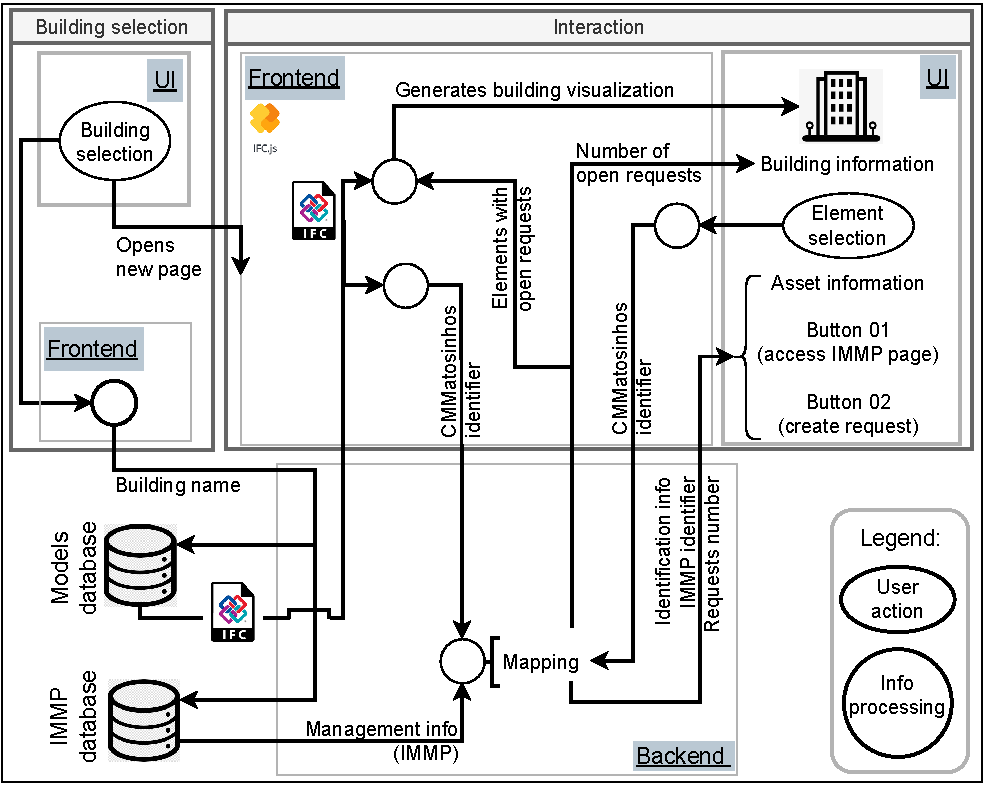
\includegraphics[width=0.48\textwidth]{Images/fluxo.pdf}
    \caption{Platform's information flow diagram}
    \label{fig_fluxo}
\end{figure}

\subsection{Unique identifiers}
\label{subsec:identifiers}

Considering the functionalities to be implemented (section \ref{sec:methodology}), three types of elements are essential to the platform's objectives: \emph{locations}, \emph{equipment} and \emph{requests}. \emph{Locations} represent spatial assets or spaces that comprise the buildings and are essential to the equipment's localization. \emph{Equipment} is any physical asset from the CMMatosinhos' inventory (vehicles, chairs, ladders, etc.). Finally, \emph{requests} represent the solicitation for an operation action to be carried out and are always associated with the other types of elements (\emph{equipment} or \emph{location}).

To establish the connections between the IMMP database and the IFC model, it is essential to comprehend how the assets are identified within the IMMP database (IMMP identifiers) and how CMMatosinhos identifies them in its inventory (CMMatosinhos identifiers). The 'CMMatosinhos identifiers' will be organized as properties to be associated with the model elements (section \ref{subsec:loin}). In contrast, the 'IMMP identifiers' will allow the mapping process between the IMMP database and the IFC model.

\paragraph{IMMP identifier}:

The IMMP database contains two categories of entries for \emph{locations}: LOCATION and ELEMENT. Within the LOCATION category, they are organized hierarchically (from buildings to zones, and to rooms) and identified by a unique attribute called 'local\_id'. On the other hand, the ELEMENT category includes two types of assets: EQUIPMENT and LOCAL. In this context, the \emph{locations} classified as ELEMENT are specifically of the type LOCAL, representing the lowest level of the spatial hierarchy found in the LOCATION category. These represent individual spaces, such as rooms. Regarding the \emph{equipment}, those are entries of the ELEMENT category and EQUIPMENT type. The 'element\_id' attribute uniquely identifies each element from the ELEMENT category. The code contained in these attributes ('local\_id' and 'element\_id') is generated automatically by the IMMP, and does not correspond to the CMMatosinhos inventory. Therefore, the 'local\_id' and 'element\_id' attributes are the IMMP identifiers for \emph{locations} and \emph{equipment}, respectively.

The \emph{requests} elements are categorized as \emph{failure} within the IMMP database, and those designated as 'open' are the relevant ones for this work since they still require actions. Since \emph{requests} are not physical assets, it was necessary to analyze their correlation with \emph{equipment} and \emph{location} elements, alongside the attributes of the \emph{failure} itself. Each request (\emph{failure}) is uniquely identified by the 'failure\_id' attribute and includes a 'local\_id' attribute that specifies the \emph{location} associated with the request. Contrarily, information regarding its connection to \emph{equipments} can only be accessed through the relationships of the \emph{equipment} elements, which allow visualization of the corresponding 'failure\_id' codes. The 'IMMP identifiers' established here are the unique identifiers for the assets in the context of the IMMP database, being a sequence of numbers (e.g. 586188) that do not represent the human-friendly identification used by CMMatosinhos.

\paragraph{CMMatosinhos identifier}:

'CMMatosinhos identifiers' refers to the coding used by CMMatosinhos to identify its assets within its inventory. This is distinct from the identifiers automatically generated by the IMMP database ('IMMP identifiers'). Each asset within the IMMP has a unique identifier specific to the IMMP but also includes the CMMatosinhos inventory code associated with one of its attributes. Among the three elements (\emph{equipment}, \emph{location}, and \emph{requests}), \emph{requests} do not have a CMMatosinhos identifier as they do not represent physical assets, being not part of CMMatosinhos' inventory.

As for \emph{locations}, the value of the 'full\_code' attribute represents the codification used by CMMatosinhos to identify spaces hierarchically, containing a unique code for each location (e.g. 009.G1.P0.048). For \emph{equipment}, the value of the 'code' attribute was selected as a potential unique identifier. Within the CMMatosinhos inventory, the value of this attribute relates to the type of equipment (e.g. \#CAD.ESCR.0056 for an office chair). However, there are cases where multiple \emph{equipment} share the same code. To address this issue, a combination of the 'code' attribute of the equipment and the 'full\_code' attribute of the location where it is situated has been defined as the 'CMMatosinhos identifier' for the equipment group. This approach considers that \emph{equipment} containing the same 'code' would not be placed in the same space.

\subsection{Level of information need}
\label{subsec:loin}

The information requirements developed in this work include the level of information need \cite{17412-1} for the model. Considering the platform features (section \ref{sec:methodology}), the model should mainly allow visualisation of the building and assets, containing only alphanumeric information relating to general building and asset information and those required for integration with the IMMP database (CMMatosinhos identifiers). Out of the three types of elements defined previously (\emph{locations}, \emph{equipment} and \emph{requests}), \emph{requests} were excluded of the level of information need definition as their visualisation and modelling is not required.

As for the elements to be modelled, three main groups of objects were defined: architectural elements, equipment and locations (table \ref{tab_loin_equipment}). In this case, the architectural elements would serve the purpose of visualisation, and only the geometrical information aspects were required for this group. For locations and equipment, geometrical and alphanumerical information requirements were defined. As for the building as a whole, since the architectural elements in table \ref{tab_loin_equipment} already cover its geometry, only alphanumerical information requirements were defined in table \ref{tab_loin_building}. For both tables (\ref{tab_loin_equipment} and \ref{tab_loin_building}) the level of information need aspects \cite{17412-1} considered non-applicable are not presented.

\begin{table*}[!htb]
    \renewcommand{\arraystretch}{2}
    \centering
    \caption{Level of information need for architectural elements, equipment and locations}
    \label{tab_loin_equipment}
    \begin{tabular}{p{0.8cm}|p{3.7cm}|p{3.2cm}p{3.2cm}p{2.0cm}}
    \hline
    \multicolumn{2}{l}{\textbf{Objects:}} & \textbf{Archit. elements} & \textbf{Equipment} & \textbf{Locations}\\
    \hline
    \multicolumn{2}{l}{\textbf{IFC Class:}} & \textbf{Variable} & \textbf{Variable} & \textbf{IfcSpace}\\
    \hline
    \multicolumn{5}{l}{\textbf{Geometrical information}} \\
    \hline
    \multicolumn{2}{l}{Detail} & Real representation of external limits. Single element without layers or components. & Simplified outer shell, real volumes and dimensions. Single element without layers or components. & Real volume.\\
    \multicolumn{2}{l}{Dimensionality} & 3D & 3D & 3D\\
    \multicolumn{2}{l}{Location} & Relative & Relative & Relative\\
    \multicolumn{2}{l}{Appearance} & Colour must be similar to reality, without textures. & Colour must be similar to reality, without textures. & Not visible\\
    \hline
    \multicolumn{5}{l}{\textbf{Alphanumerical information}} \\
    \hline
    \multicolumn{5}{l}{Attributes} \\
    \hline
    & Attribute name & \multicolumn{3}{c}{Content}\\
    \hline
    & LongName & X & X & Name\\
    \hline
    \multicolumn{5}{l}{Properties} \\
    \hline
    Group & Property name & \multicolumn{3}{c}{Content}\\
    \hline
    \multirow{4}{*}{**} & Codigo\_CMMatosinhos & X & Code & X\\
    & Local\_CMMatosinhos & X & X & Code\\
    & Categoria\_CMMatosinhos & X & Category & X\\
    & Tipo\_CMMatosinhos & X & Category description & X\\
    \hline
   \multirow{6}{*}{\rotatebox{90}{\textbf{Legend}}} & \multicolumn{4}{l}{\textbf{Variable}}\\
    & \multicolumn{4}{l}{    IFC classes vary depending on the architectural element or equipment.}\\
    & \multicolumn{4}{l}{\textbf{**}}\\
    & \multicolumn{4}{l}{    Name fo group of properties: CMMatosinhos\_Identification}\\
    & \multicolumn{4}{l}{\textbf{X}}\\
    & \multicolumn{4}{l}{    Objects of this type must not contain this property or attribute.}\\
    \hline
    \end{tabular}
\end{table*}

\begin{table*}[!htb]
    \renewcommand{\arraystretch}{2}
    \centering
    \caption{Level of information need for the building}
    \label{tab_loin_building}
    \begin{tabular}{p{5.1cm}|p{4.3cm}|p{4.3cm}}
    \hline
    \textbf{Objects:} & \multicolumn{2}{l}{\textbf{Building}}\\
    \hline
    \textbf{IFC Class:} & \multicolumn{2}{l}{\textbf{IfcBuilding}}\\
    \hline
    \multicolumn{3}{l}{\textbf{Alphanumerical information}} \\
    \hline
    \multicolumn{3}{l}{Attributes} \\
    \hline
    & Attribute name & Content\\
    \hline
    & LongName & Name\\
    \hline
    \multicolumn{3}{l}{Properties} \\
    \hline
    Group & Property name & Content\\
    \hline
    CMMatosinhos\_Identification & Local\_CMMatosinhos & Code\\
    \hline
    \end{tabular}
\end{table*}

\subsection{Web platform}
\label{subsec:platform}

Figure \ref{fig_plataforma} shows screenshots of the web platform from the perspective of a user of the manager type. Screenshot A shows the interaction page after a building is selected and the model is loaded, presenting a 3D view of the entire building. When an asset is selected, the platform will appear as screenshot B. The interaction page includes an upper section (screenshot C) presenting the building's identification and the possibility of editing the visualization mode, whether by floor or entire building, whether all elements or only those with open requests. The next section (screenshot D) warns about the presence and number of open requests associated with the building. The side menu (screenshot E) displays information about the selected asset, and it appears on the user interface only when a piece of equipment or space is selected. In this menu, it is possible to visualize information identifying the selected asset and the number of associated open requests. In addition, two buttons allow the redirection to the asset's page within the IMMP and the creation of requests (screenshot F) associated directly with the asset. The request is automatically registered within the IMMP platform.

\begin{figure*}[!htb]
    \centering
    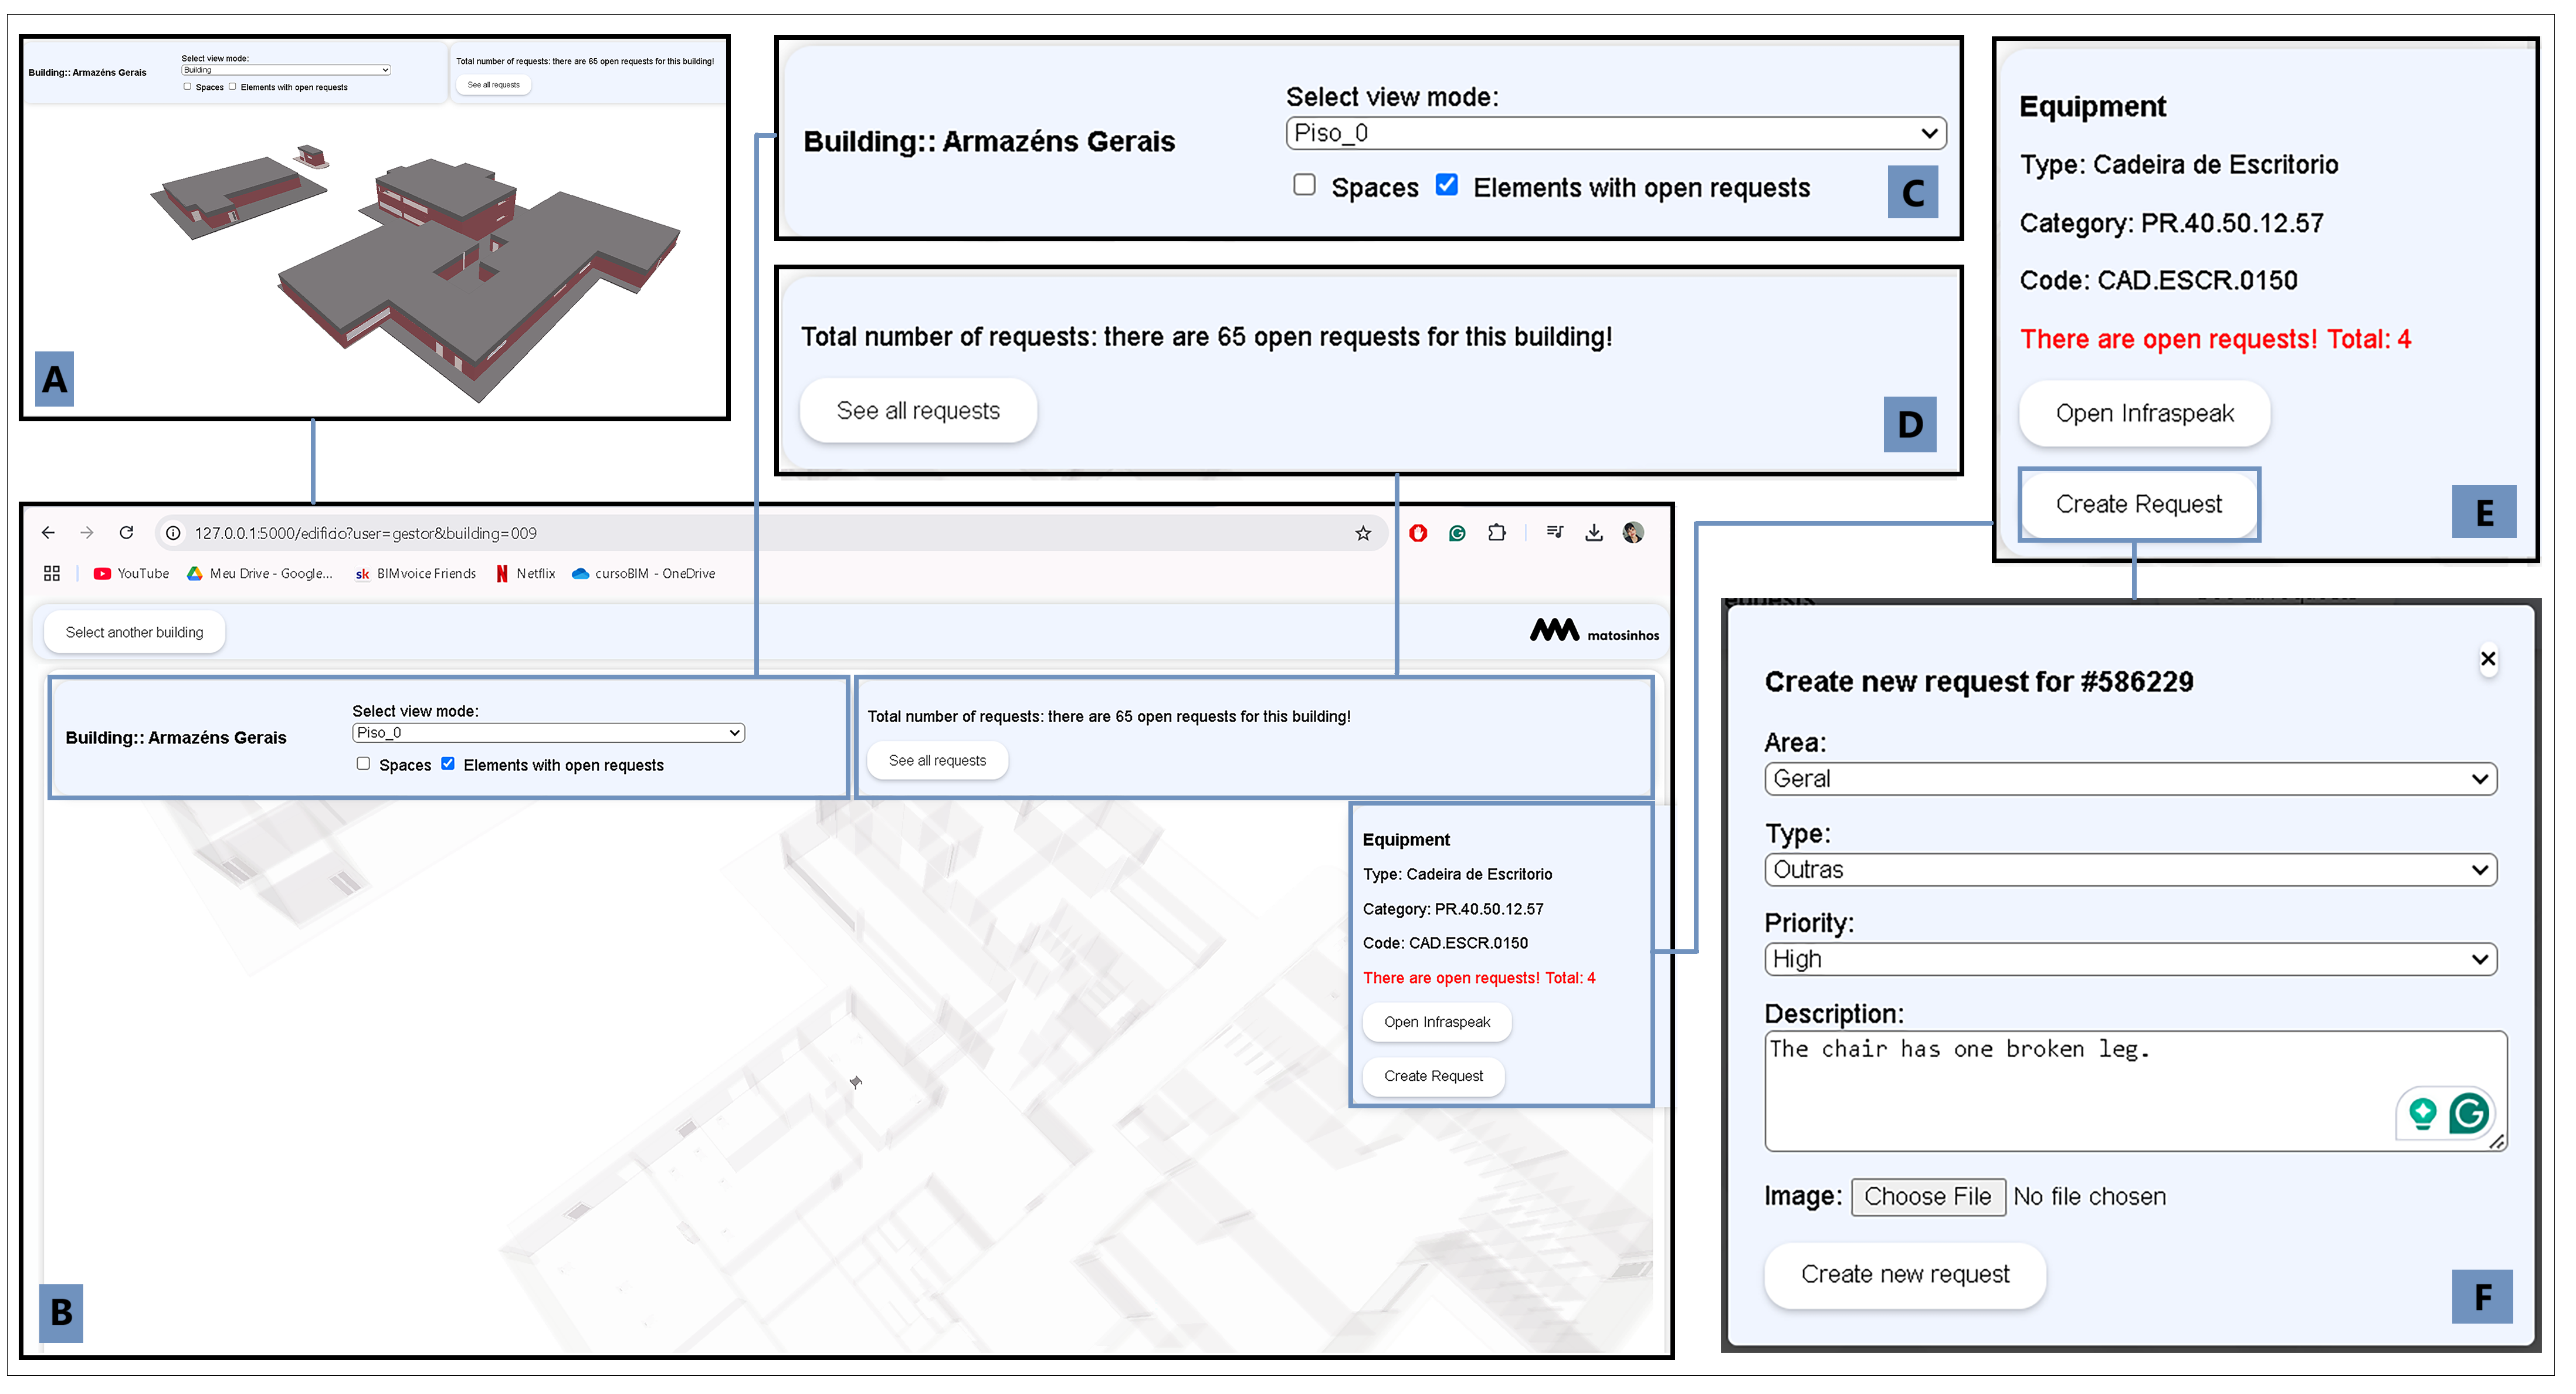
\includegraphics[width=\textwidth]{Images/plataforma.png}
    \caption{Web platform}
    \label{fig_plataforma}
\end{figure*}

\section{Discussion and conclusion}
\label{sec:conclusion}

This work demonstrated the development and implementation of a BIM-based solution for FM, which has been integrated with an existing management platform that previously did not support BIM. Additionally, the outcomes of this work provide a framework for future integration processes. This partnership illustrates that the operational section does not need to rebuild its management system from the ground up or adopt a different platform to effectively implement BIM. However, it does need to organize its inventory to facilitate digitalization. An iterative process with CMMatosinhos helped to address limitations encountered during development, resulting in optimizations that enhanced the user experience. The use of the IFCjs library enabled various visualization modes for the models and allowed for data extraction to support integration with the IMMP platform.

\section{Acknowledgements}
\label{sec:acknowledgements}

This work was partly financed by FCT / MCTES through national funds (PIDDAC) under the R\&D Unit Institute for Sustainability and Innovation in Structural Engineering (ISISE), under reference UIDB / 04029/2020 (doi.org/10.54499/UIDB/04029/2020), and under the Associate Laboratory Advanced Production and Intelligent Systems ARISE under reference LA/P/0112/2020. This work is also financed by national funds through FCT – Foundation for Science and Technology, under grant agreement PRT/BD/154416/2023 attributed to the 1st author, under the MIT Portugal Programme.

\bibliography{ISARC}

\end{document}
